An alternative ADC solution is to adapt the ADC chip under development for the 
ATLAS liquid argon calorimeter readout upgrade for the HL-LHC.  The main ATLAS 
requirements are given in Table~\ref{tab:ATLAS-ADC-reqs}.  Adapting the chip to DUNE needs 
would require doubling the number of channels per chip as well as adapting the output 
architecture.  These are both relatively simple changes compared to the overall complexity of the chip.

\begin{dunetable}
[Performance requirements for the ATLAS-style ADC ASIC.]
{ll}
{tab:ATLAS-ADC-reqs}
{Performance requirements for the ATLAS-style ADC ASIC.}
\textbf{Parameter} &\textbf{Specification}\\ \toprowrule
Channels/chip & 8 preferred, 4 minimum \\ \colhline
Sampling Frequency & \SI{40}{MHz} \\ \colhline
Dynamic Range & \SI{14}{bits}  \\ \colhline
Precision & \SI{11}{ENOB}\\ \colhline
Power & $<$~\SI{100}{mW}/channel at \SI{40}{MHz}\\ \colhline
Input & \SI{2}{V} differential\\ \colhline
Output & E-link interface operating at \SI{640}{Mbps}\\
\end{dunetable}

To achieve a 14-bit dynamic range, each analog channel is comprised
of two main sections: a Dynamic Range Enhancement (DRE) block that determines the
most significant two bits of the 14-bit digital code, followed by a 12-bit SAR block. %The design of the DRE is shown schematically in Figure~\ref{fig:65nmADCarchitecture_dre}.
The input signal to the DRE block is sampled on two
paths, one with unity gain and the other of gain four. A comparator determines which gain to use.
The signal from the selected DRE gain is presented at the DRE output,
which is connected to the input of the 12-bit SAR ADC block. The DRE design has been carefully
optimized so that its output preserves the required 12-bit performance.

%\begin{dunefigure}
%[Block diagram of the DRE architecture for the ATLAS ADC ASIC.]
%{fig:65nmADCarchitecture_dre}
%{Block diagram of the DRE architecture for the ATLAS ADC ASIC.}
%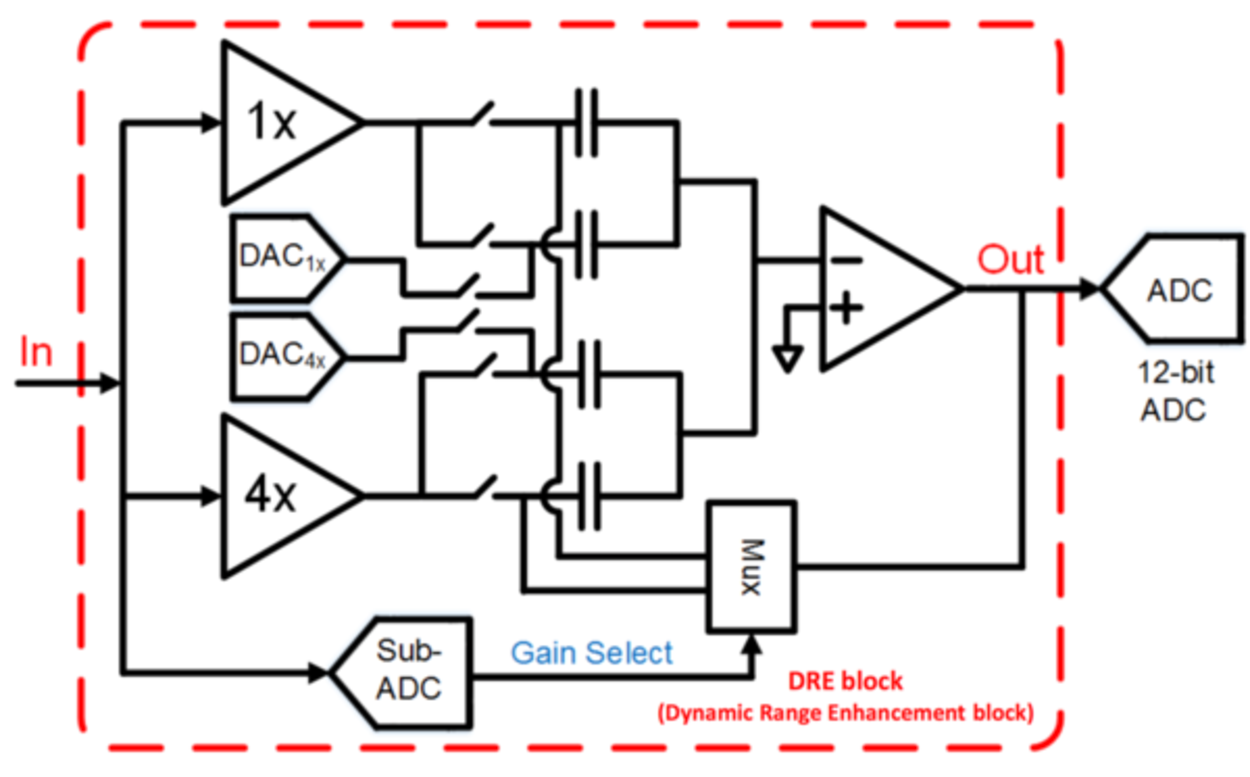
\includegraphics[width=.55\textwidth]{tpcelec-DREconcept_resized.pdf}
%\end{dunefigure}

Following current state-of-the-art ADC development techniques, a two-stage 
SAR architecture is used, exploiting the high speed of the technology while maintaining the SAR input 
capacitance at a reasonable value. Since capacitor matching in this technology might not meet the 
precision required, the ADC will use bit redundancy, i.e.~determine more bits than its actual output, 
and the redundant bits will be used to both calibrate the ADC and produce correct output codes. 
Such procedures are well understood and applied to both pipeline~\cite{Kuppambatti:2013nfa} and 
SAR~\cite{5999734} ADCs using foreground or background calibration techniques. Details of the SAR design are shown in Figure~\ref{fig:65nmADCarchitecture_sar}. 

\begin{dunefigure}
[Block diagram depicting the two-stage SAR design of the ATLAS ADC ASIC.]
{fig:65nmADCarchitecture_sar}
{Block diagram depicting the two-stage SAR design of the ATLAS ADC ASIC.}
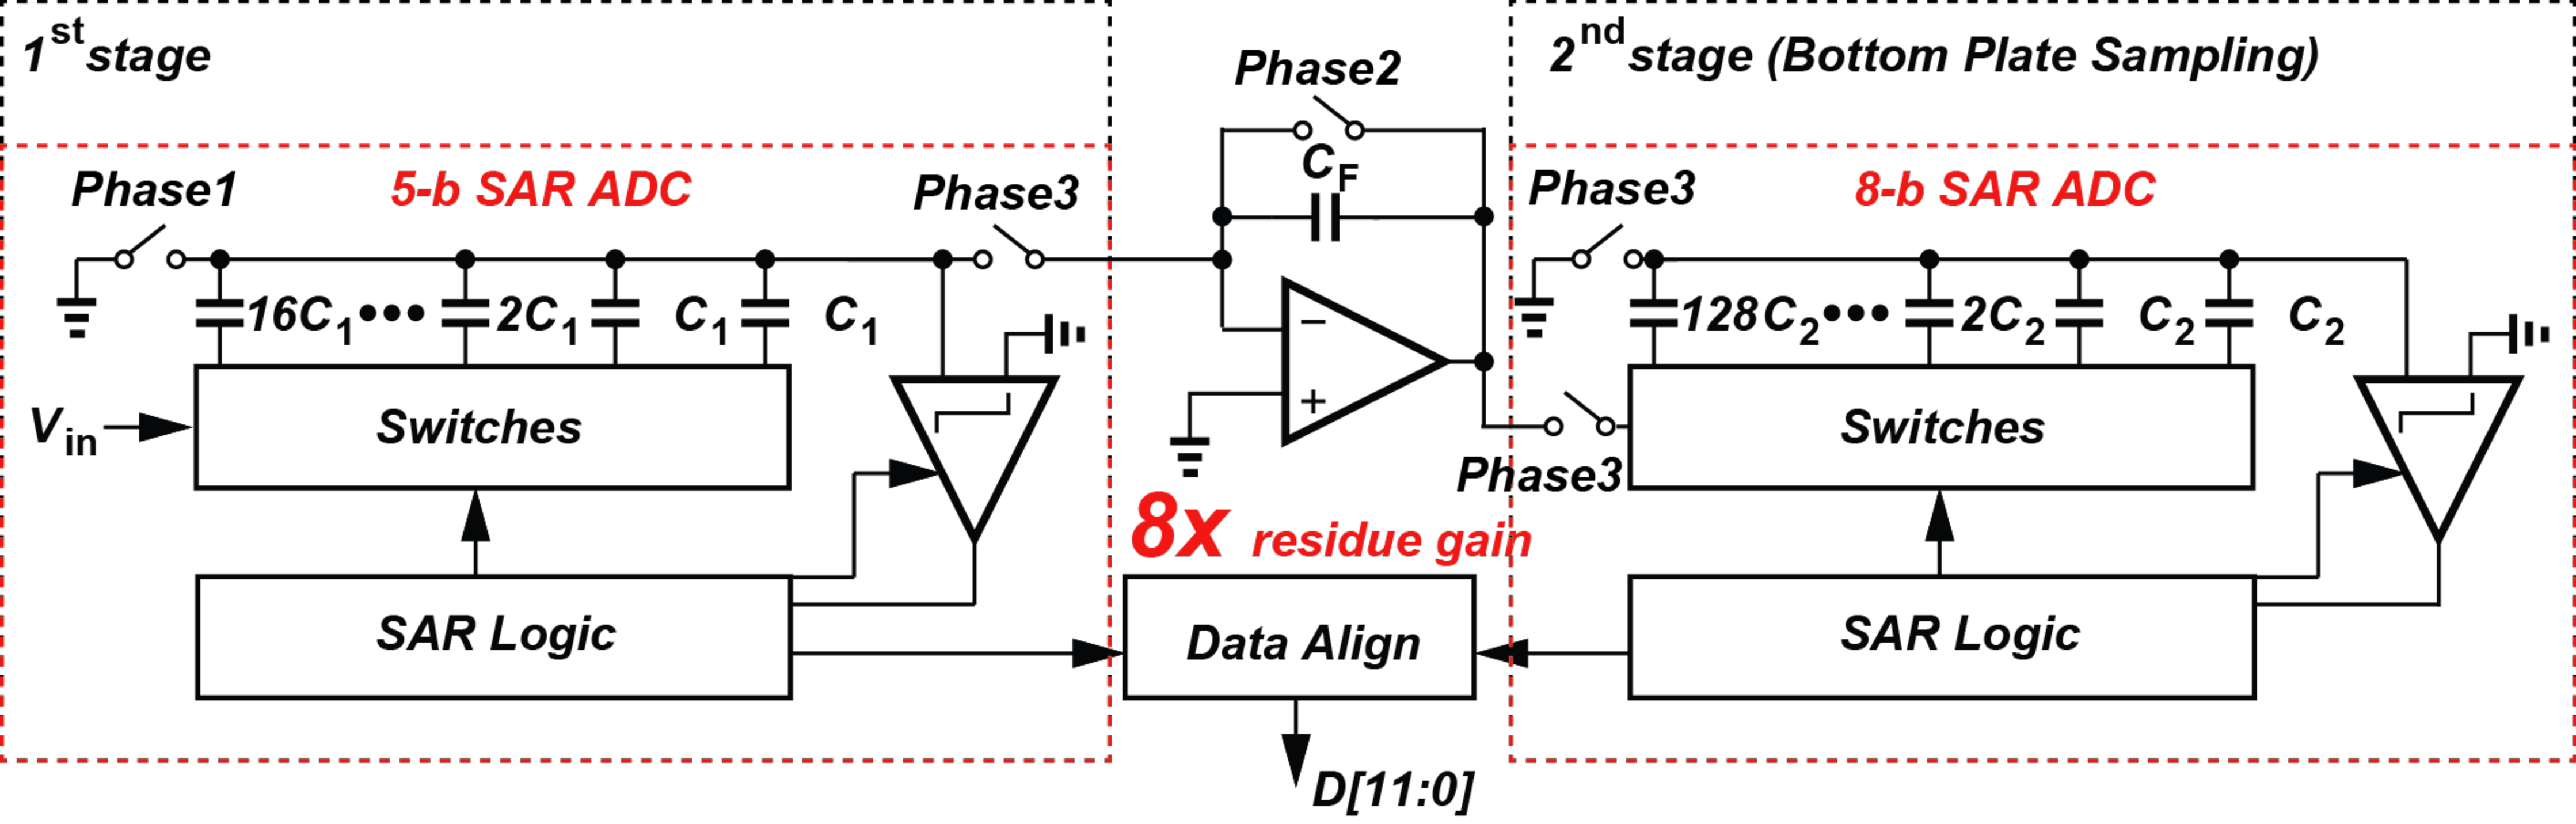
\includegraphics[width=.9\textwidth]{tpcelec-SARdesign.pdf}
\end{dunefigure}

An ADC test chip, dubbed COLUTA65V1, was designed and submitted for fabrication in May 2017 and received
in September of 2017.  The DRE and SAR blocks of the COLUTA65V1 were first tested independently. Measurements were made of the SAR precision using the sine-wave Fast Fourier Transform method. An effective number of bits
(ENOB) of \SI{11.6}{bits} at \SI{20}{MHz} (after calibration) was obtained.
%Similar measurements at \SI{40}{MHz} do not match the expected performance and 
%additional testing and simulation indicates that the layout of the connection between the first SAR stage and the amplifier is not optimal. Similar results were observed with
%the DRE performance and again simulation indications improvements are possible in the layout. 
%The next submission of the chip, planned for Spring 2018, will incorporate this work in the iteration 
%of the design.
Both DRE and SAR were successfully integrated with negligible degradation in performance. The COLUTA65V1 chip was also tested at 2~MHz and shown to work as designed, meeting the requirement for DUNE. Tests of an updated design in liquid nitrogen are planned for Spring 2018. Additional tests associated with meeting power requirements will be carried out if this ADC option is further pursued.
